\chapter{科技文档}

\begin{quote}
    智慧人积存知识,愚妄人的口速致败坏。——《圣经·箴言》10:14
\end{quote}

现在,终于到了跟你聊聊所谓\emph{科技}文档特性的时刻。虽然关于数学式和其他方程的问题已经在第3章妥善解决,但还有一块骨头要啃:参考文献。对于这个问题,虽然不能一口吃个胖子,但接下来的内容可以让你大幅简化工作。在本章,我们还会解释生成索引的机制。

本章首先会介绍起草文章的几点特别之处,然后展示参考文献的生成和索引的生成,最后介绍将大篇幅文档拆解成几个小部分的实用方法。

\section{文章(article)}

为了起草一篇文章,没有什么新内容可以介绍的,我们目前为止见过的所有内容都适用。只需要注意,在文前部分中,可以使用以下指令:

\begin{itemize}
    \item \verb|\title|,定义标题;
    \item \verb|\date|,定义日期;
    \item \verb|\author|,定义作者团队;
    \item \verb|\thanks|,定义作者单位。
\end{itemize}

若要利用这些定义来插入标题,需要在\verb|\begin{document}|之\textbf{后}插入指令\verb|\maketitle|:

\begin{dmd}
\begin{verbatim}
\documentclass{article}
\title{Le seuillage à 128 : une révolution !}
\author{M. C. Orlanrien\\
        Institut du Pixel\\
        42007 Saint-Etienne---FRANCE}
\date{2 Avril 1927}
\begin{document}
\end{verbatim}
\backslash maketitle\textsl{\% 标题插到此处}\\
...\\
\verb|\end{document}|
\end{dmd}

此处重复一遍\jz{
    因为传授知识就是重复的过程。
}:标题是由指令\verb|\maketitle|生成并插入的,而不是文前部分的定义。

通常来说,会议或期刊提供的模板文件中会引入一些变化(例如使用\verb|\address|分隔作者和其地址),但基本原理是一致的。

\section{参考文献}

由两种方式可以使用\LaTeX 起草文章的参考文献部分。其中,可以称得上是“手动”的方式是,在文章中插入环境\dm{thebibliography}。另一种方式,即此处要介绍的方式,是使用\bib ,主要分为如下步骤。

\begin{enumerate}
    \item 创建一个或多个参数文件,包含\bib 格式的各条参考文献入口(entrée;文章、会议……)。这个步骤不可避免地需要我们去\emph{输入}。
    \item 在文档中,使用指令\verb|\cite|去引用这些入口。
    \item 参考文献会自动根据你选择的特殊风格排版。
\end{enumerate}

这种方法的优势是,对于每条参考文献,你只需输入一次。此外,考虑到可以使用\emph{风格文件},你不用去担心它的版式。有几十种风格文件,对应各种标准,包含期刊和其他会议所使用的标准。我们也可以在互联网上找到\bib 格式的参考文献数据库,可以在文档中直接使用。

我们重复一遍:参考文献有多种标准。但不幸的是,一些期刊偏偏喜欢指定属于自己的参考文献格式。有朝一日你在这种期刊上发表文章时,就需要去创建或调整风格文件。为了实现这一点,可以去查找工具\textsf{makebst}。

\subsection{\dm{.bib}文件}

第一个操作是构建\jz{
    \textbf{Emacs}的Auc\TeX 组件包含了很好用的\bib 模式。
}参考文献文件,其扩展名最好为\dm{.bib}。该文件需要遵循特殊的语法。首先需要知道,\bib 通过\emph{类型(type)}区分每个入口。这样一来,每个入口都带有一个文档类型:图书、文章、会议、科技报告……一共有二十多种不用的文档类型。

\begin{ii}
正常来说,我们可以在伴随\LaTeX 发行版提供的文件找到名为\bib ing的文件(命名为\dm{btxdoc.pdf}),由奥兰·帕塔什尼克(Oran Patashnik)在约二十年前创作。该文件包含有关构建\bib 格式文件方法的重要信息来源。
\end{ii}

每个入口\emph{类型}都包含一定数量描述该入口的\emph{字段(champ)}。参考文件入口的结构如下:

\begin{dmd}
@\codereplace{入口}\{\codereplace{关键描述},\\
\verb|  |\codereplace{字段$_1$}\ =\ \{...\},\\
\verb|  |\codereplace{字段$_2$}\ =\ \{...\},\\
\verb|  |...\\
\verb|  |\codereplace{字段$_n$}\ =\ \{...\},\\
\}
\end{dmd}

其中,\codereplace{入口}表示文档类型(\dm{article}、\dm{inproceedings}等),\codereplace{字段$_1$}、\codereplace{字段$_2$}……\codereplace{字段$_n$}表示参考文献入口的不同字段。这些\bib 的保留字可以以大写或小写形式输入。

符号\codereplace{关键描述}需要以唯一方法描述该文档,以备通过用于识别标签的符号\verb|\label|来重新找到。为了你能够快速上手\bib ,接下来的示例综合了三个你需要使用的基本入口。

\subsubsection{期刊文章}

有一篇期刊文章需要以如下形式输入:

\begin{dmd}
\begin{verbatim}
@article{qtz:UchArb,
    author ={Uchiyama, Toshio and Arbib, Michael A.},
    title = {Color Image Segmentation
            Using Competitive Learning},
    journal=pami,
    volume =16, number=2, pages={1197--1206},
    month=dec, year=1994}
\end{verbatim}
\end{dmd}

有以下几点需要注意。

\begin{enumerate}
    \item 字段\dm{author}、\dm{title}、\dm{journal}、\dm{year}是必需的。
    \item 对于作者\jz{
        此处关于作者的注意事项对于其他入口(会议、书等)也同样适用。
    }姓名,需要遵循\codereplace{姓}、\codereplace{名}的顺序。\textbf{所有}作者姓名都需要以\dm{and}分隔。
    \item 对于复合姓或其他特殊作者名,可以以如下形式输入:
    \begin{center}
        \dm{author="de la Motte Beuvron, Alain"}
    \end{center}
    其中遵循的顺序为:\codereplace{特殊组成部分}、\codereplace{姓}、\codereplace{名}。逗号作为分割符,起到与上例中相似的作用。
    \item 所有月份可以以字符串的形式给出,如\dm{jan}、\dm{feb}、\dm{mar}等。
\end{enumerate}


在\dm{.bib}文件的开头,为简洁起见,我们已经创建了\emph{缩写}\dm{pami}:

\begin{dmd}
\begin{verbatim}
@string{pami="IEEE transactions on Pattern Analysis and
              Machine Intelligence"}
\end{verbatim}
\end{dmd}

\subsubsection{会议析出文章}

没错,\bib 会区分对待\emph{期刊}和\emph{会议}中的文章。格式结构与上例很相似,只不过\dm{booktitle}用于会议标题而不是期刊标题:

\begin{dmd}
\begin{verbatim}
@Inproceedings{qtz:BouOrch,
    author={Bouman, Charles A. and Orchard, Michael T.}
    title={Color Image Display with a Limited Palette Size},
    booktitle={SPIE Conference on Visual Communications
               and Image Processing},
    volume=1199,pages={522--533},
    year=1989}
\end{verbatim}
\end{dmd}

这里,\dm{author}、\dm{title}、\dm{booktitle}、\dm{year}是必填字段,我们可以选用\dm{volume}和\dm{number}。

\subsubsection{图书片段}

相比于整本书,我们经常指参考其中的一个片段——若干章、若干页:

\begin{dmd}
\begin{verbatim}
@inBook{col:McA,
    author =    {MacAdam, David L.},
    title =     {Color Measurement},
    chapter =   4,
    pages   =   {48--49},
    publisher = {Springer-Verlag},
    year =      1985}
\end{verbatim}
\end{dmd}

强制字段为:\dm{author}、\dm{title}、\dm{chapter}或\dm{pages}、\dm{publisher} (出版方),以及\dm{year}。

\begin{ii}
我们再次强烈建议你使用Emacs组件Auc\TeX 的\textsc{Bib}\TeX 模式。特别是该模式为你提供了包含所有入口类型的菜单。选择菜单中的一项,就可以在你的文件中插入入口“骨架”。该组件可以在\wz{ftp.lip6.fr/pub/TeX/CTAN/support/auctex}下载,也可以以包Debian的形式获取。
\end{ii}

\subsection{参考文献的标注}

一旦参考文献建立完成,就可以即刻在文档中借助关键描述使用指令\verb|\cite|来标明引用:

\begin{dmd}
\backslash cite\{\codereplace{关键描述}\}
\end{dmd}

指令\verb|\cite|有如下功能:

\begin{enumerate}
    \item 根据选择的风格插入跳转符号(如[2]、[Loz95]等);
    \item 在文档的参考文献部分中添加所引用的文章。
\end{enumerate}

\begin{ii}
    文章(此处指广义的文章)只有在被\verb|cite|作为引用对象时才会出现在参考文献中。若要列出未于正文中直接引用的文章,则需要使用指令\verb|\nocite{|\codereplace{关键描述}\verb|}|将\codereplace{关键描述}的对应文章插入文档的参考文献部分。此外,指令\verb|\nocite{*}|会将\dm{.bib}文件中的\emph{所有}入口插入文档。
\end{ii}

在实际进入生成参考文献的步骤前,需要在\LaTeX 文档末尾添加对以下指令的引用来指定参考文献的风格:

\begin{dmd}
\verb|\bibliographystyle|
\end{dmd}

然后,引用如下指令来实际插入参考文献:

\begin{dmd}
\verb|\bibliography|
\end{dmd}

对于风格,有:

\begin{dmd}
\backslash bibliographystyle\{\codereplace{风格}\}
\end{dmd}

\LaTeX 预定义的风格\jz{
    在CTAN网站的\dm{biblio/bibtex/contrib}可以找到几十种可供使用的其他风格。
}如下。

\begin{itemize}
    \item \dm{plain},引用的形式为[2],参考文献会根据作者名排序。
    \item \dm{unsrt},参考文献根据引用顺序排序。会议文章经常使用这种风格。
    \item \dm{alphs},引用的形式为“作者缩写+年份”。
\end{itemize}

接下来,需要指定哪些文件包含了文档中指令\verb|\cite|所“指向”的那些参考文献:

\begin{dmd}
\backslash bibliography\{\codereplace{文件$_1$}, \codereplace{文件$_2$}, \codereplace{……}\}
\end{dmd}

这样的指令会使\bib 在处理过程中包含\codereplace{文件$_1$}\dm{.bib}、\codereplace{文件$_2$}\dm{.bib}……

\subsection{生成参考文献}

生成参考文献的步骤如下。

\begin{enumerate}
    \item 借助\LaTeX 实现第一次编译,使得辅助文件\dm{doc.aux}包含\emph{引用标注}信息:
    
    \begin{center}
        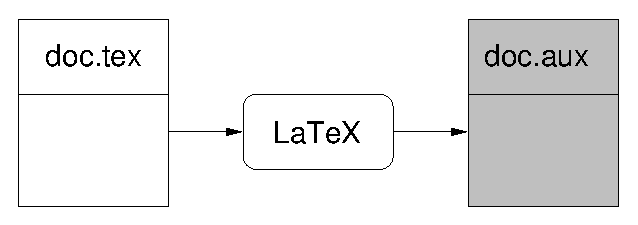
\includegraphics{img/bibtex1}
    \end{center}
    
    \item 运行\bib ,在文件\dm{doc.bbl}中生成参考文献:
    
    \dmh{bibtex doc}

    \begin{center}
        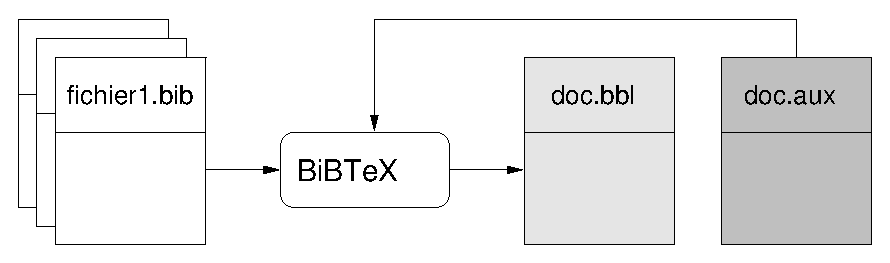
\includegraphics{img/bibtex2}
    \end{center}

    \item 借助\LaTeX 的第二次编译插入参考文献:
    
    \begin{center}
        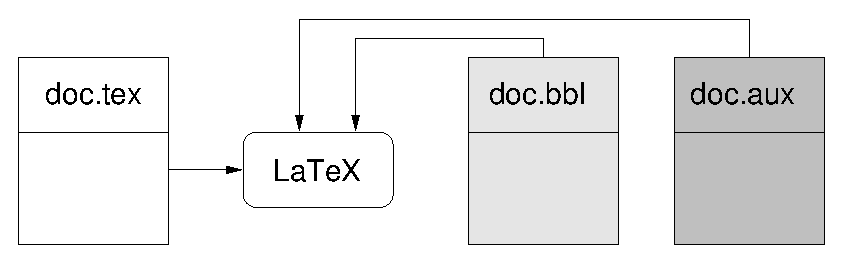
\includegraphics{img/bibtex3}
    \end{center}

    %TODO 图片中bibtex和latex替换

    \item 通过第三次编译解析交叉引用。
\end{enumerate}

如果你对这个过程感到好奇,可以看到:文件\dm{doc.bbl}包含了环境\dm{thebibliography}以供随时使用\jz{
    也就是说,你如果不使用\bib ,就必须着手处理该环境。
};文件\dm{doc.blg}是与那些\dm{.log}文件相似的“日志”文件,储存着上一次使用\bib 时一些可能出现的错误或警告。

\begin{exclamation}
程序\bib 对环境\dm{BIBINPUTS}中的参数敏感。因此,在某些情况下,有必要在\linebreak\dm{.bash\_profile}中添加以下一行命令:

\dmh{export BIBINPUTS=\$HOME/LaTeX/biblio//:}

这样可以使\bib 在目录\dm{\$HOME/LaTeX/biblio}中搜索你的参考文献文件(此处的目录为示例)。
\end{exclamation}

\section{索引}

生成索引需要依靠以下两个概念:

\begin{enumerate}
    \item 在\LaTeX 文档中添加指令\verb|\index|来添加索引入口;
    \item 使用程序\textbf{makeindex}来正确地抽取和展示索引。
\end{enumerate}

负责在文档中插入索引部分的是指令\verb|\printindex|。可以将该指令与\verb|\tableofcontents|类比。

\subsection{必要步骤}

这里给出简短的索引制作备忘录:

\begin{enumerate}
    \item 在主文件中插入两条指令:
    \begin{dmd}
    \begin{tabbing}
12345678902234567890\=\kill
\verb|\makeindex|\>\textsf{$\leftarrow$告知\LaTeX 需要生成索引}\\
\verb|\begin{document}|\\
{\rmfamily ……文档正文……}\\
\verb|\printindex|\>\textsf{$\leftarrow$在文档中实际插入索引部分}\\
\verb|\end{document}|
    \end{tabbing}
    \end{dmd}

    \item 插入索引入口:
\begin{dmd}
\begin{tabbing}
12345678902234567890\=\kill
\verb|\index{bidule}|\>\textsf{$\leftarrow$在索引中插入“bidule”}
\end{tabbing}
\end{dmd}

    \item 为了为文档\dm{doc.tex}生成索引,需要成功执行以下三条指令:
    
    \begin{dmd}
        latex doc\\makeindex doc\\latex doc
    \end{dmd}
\end{enumerate}

\subsection{机制细节}

文档\dm{doc.tex}的第一次编译(在满足文前部分带有控制序列\verb|\makeindex|的条件下)会生成包含“散装”的索引入口文件\dm{doc.idx}:

\begin{center}
    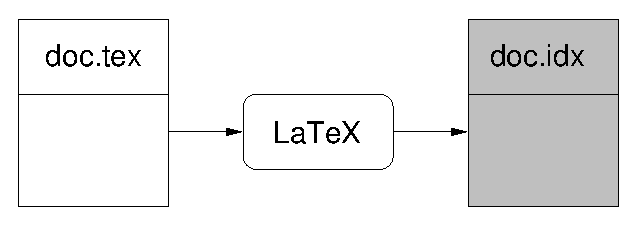
\includegraphics{img/makeindex1}
\end{center}

接下来,使用\textsf{makeindex},在这个文件\dm{doc.idx}中整理条目、删除重复项,并将结果存入\dm{doc.ind}。执行轨迹会存储在\dm{doc.ilg}中:

\begin{center}
    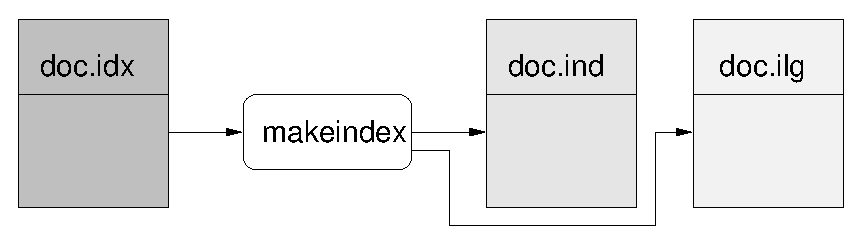
\includegraphics{img/makeindex2}
\end{center}

终端下运行的\textsf{makeindex}嘴很碎。如下展示了它生成文档索引时展示的信息:

\begin{dmd}
\begin{verbatim}
This is makeindex, version 2.13 [07-Mar-1997] (using kpathsea).
Scanning input file guide.idx....done (982 entries accepted, 0 rejected).
Sorting entries...........done (11254 comparisons).
Generating output file guide.ind....done (745 lines written, 0 warnings).
Output written in guide.ind.
Transcript written in guide.ilg.
\end{verbatim}
\end{dmd}

因此,在运行失败的情况下,需要警惕可能出现的抛出和警告(\emph{warning})。\LaTeX 的第二次编译可以在\dm{doc.tex}中指令\verb|\printindex|指出的位置插入格式化过的索引(文件\dm{doc.ind}):

\begin{center}
    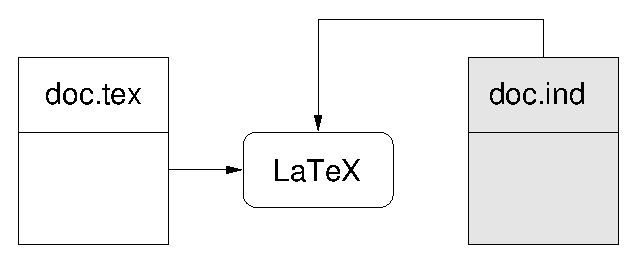
\includegraphics{img/makeindex3}
\end{center}

\begin{ii}
工具makeindex可以识别选项\dm{-s},该选项用于为索引指定\emph{风格}。这里所说的风格定义在带有扩展名\dm{.ist}的文件中,可以改变索引的排版央视。可以以如下方式修改文件风格:

\dmh{makeindex -s}\codereplace{文件风格}\codereplace{主文件}

可以在你使用的发行版中寻找风格文件并测试它们。
\end{ii}

\subsection{索引入口的不同类型}

目前为止,我们看到的索引形式都是\emph{\codereplace{索引词}及\codereplace{页码}},但也可以使用更讲究些的入口形式,至少包含如下三种。

\begin{enumerate}
    \item 带有层级的入口:
    
    \begin{dmd}
    \verb|\index{bidule!chouette}|
    \end{dmd}

    该指令可以在索引中插入“bidule”的子入口“bidule”。

    \item 跨页入口:
\begin{dmd}
\begin{tabbing}
12345678902234567890\=\kill
\verb+\index{bidule|(}+\>\textsf{$\leftarrow$位于第$i$页}\\
\verb+\index{bidule|)}+\>\textsf{$\leftarrow$位于第$j$页}
\end{tabbing}
\end{dmd}
    该指令插入的索引形式为bidule $i$--$j$。

    \item 符号化的入口:
    
    \begin{dmd}
    \verb|\index{alpha@\alpha}|
    \end{dmd}

    这样的指令会在索引中插入$\alpha$,并按“alpha”将其分类。同样地,以下指令会在索引中插入“épluche”,但分类时会将首字母看作“e”:

    \begin{dmd}
    \verb|\index{eplucher@éplucher}|
    \end{dmd}
\end{enumerate}

此处列出的最后一个格式同样可以用于为索引插入带有特殊版式的入口。例如:

\begin{dmd}
\verb|\index{bonjour@\textbf{bonjour}}|
\end{dmd}

该指令可以在索引中插入\textbf{bonjour}(即将bonjour加粗),同时按“bonjour”将该入口分类。